\documentclass[twoside]{article}

\usepackage{lipsum}
\usepackage[none]{hyphenat} 

\usepackage[sc]{mathpazo} 
\usepackage[T1]{fontenc} 
\linespread{1.05}
\usepackage{microtype}

\usepackage[hmarginratio=1:1,top=32mm,columnsep=20pt]{geometry}
\usepackage{multicol} 
\usepackage[hang, small,labelfont=bf,up,textfont=it,up]{caption} 
\usepackage{booktabs} 
\usepackage{float} 
\usepackage[hidelinks]{hyperref} 
\usepackage[usenames]{color}

\usepackage{lettrine} 
\usepackage{paralist}

\usepackage{abstract} 
\renewcommand{\abstractnamefont}{\normalfont\bfseries}
\renewcommand{\abstracttextfont}{\normalfont\small\itshape} 

\usepackage{titlesec} 
\renewcommand\thesection{\Roman{section}} 
\renewcommand\thesubsection{\Roman{subsection}} 
\titleformat{\section}[block]{\large\scshape\centering}{\thesection.}{1em}{} 
\titleformat{\subsection}[block]{\large}{\thesubsection.}{1em}{}

\usepackage{fancyhdr} 
\pagestyle{fancy} 
\fancyhead{} 
\fancyfoot{}

\fancyhead[C]{ Simulaci\'on $\bullet$ Programaci\'on Declarativa $\bullet$ Agentes-Haskell}
\fancyfoot[RO,LE]{\thepage}

\title{\vspace{-15mm}\fontsize{20pt}{10pt}\selectfont\textbf{Proyecto de Simulaci\'on y Programaci\'on Declarativa}}

\author{
\large
\textbf{\large Agentes-Haskell} \\[1.5cm]
\textsc{Alejandro Campos. C-411}\\\\[2mm]
\normalsize Facultad de Matem\'atica y Computaci\'on \\
\normalsize Universidad de la Habana \\
\normalsize 2021 \\[2cm]
\vspace{-5mm}
}
\date{}


\usepackage{graphicx}
\begin{document}

\maketitle

\thispagestyle{fancy} 


\section{Introducci\'on}
Un agente es un sistema computacional situado dentro de un medio ambiente, dentro del cual es capaz de realizar acciones aut\'onomas encaminadas a lograr sus objetivos. Un agente inteligente es aquel que es capaz de ejecutar aut\'onomas flexibles para lograr sus objetivos, donde flexible significa: reactivo, proactivo y sociable. Se define reactivo como que el agente es capaz de percibir su ambiente y responder de un modo oportuno a los cambios que ocurren para lograr sus metas. Proactivo quiere decir que debe ser capaz de mostrar un comportamiento dirigido a objetivos tomando la iniciativa para lograrlos. Por \'ultimo, un agente sociable debe ser capaz de interactuar con otros agentes para lograr sus prop\'ositos. 

El problema de agentes en el cual se centra el proyecto se detalla a continuaci\'on:\\

El ambiente en el cual intervienen los agentes es discreto y tiene la forma de un rect\'angulo de N x M. El ambiente es de informaci\'on completa, por tanto, todos los agentes conocen toda la informaci\'on sobre el agente. El ambiente puede variar aleatoriamente cada t unidades de tiempo. El valor de t es conocido. Las acciones que realizan los agentes ocurren por turnos. En un turno, los agentes realizan sus acciones, una sola por cada agente, y modifican el medio sin que este var\'ie a no ser que cambie por una acci\'on de los agentes. En el siguiente, el ambiente puede variar. Si es el momento de cambio del ambiente, ocurre primero el cambio natural del ambiente y luego la variaci\'on aleatoria. En una unidad de tiempo ocurren el turno del agente y el turno de cambio del ambiente. Los elementos que pueden existir en el ambiente son obst\'aculos, suciedad, ni\~nos, el corral y los agentes que son llamados Robots de Casa. A continuaci\'on se precisan las caracter\'isticas de los elementos del ambiente:

Obst\'aculos: Estos ocupan una \'unica casilla en el ambiente. Ellos pueden ser movidos, empuj\'andolos, por los ni\~nos, una \'unica casilla. El Robot de Casa, sin embargo, no puede moverlo. No pueden ser movidos por ninguna de las casillas ocupadas por cualquier otro elemento del ambiente.

Suciedad: La suciedad es por cada casilla del ambiente. Solo puede aparecer en casillas que previamente estuvieron vac\'ias. Esta, o aparece en el estado inicial o es creada por los ni\~nos.

Corral: El corral ocupa casillas adyacentes en n\'umero igual al del total de ni\~nos presentes en el ambiente. El corral no puede moverse. En una casilla del corral solo puede coexistir un ni\~no. En una casilla del corral, que est\'e vac\'ia, puede entrar un robot. En una misma casilla del corral pueden coexistir un ni\~no y un robot solo si el robot lo carga, o si acaba de dejar al ni\~no.

Ni\~no: Los ni\~nos ocupan solo una casilla. Ellos en el turno del ambiente se mueven, si es posible (si la casilla no est\'a ocupada: no tiene suciedad, no est\'a el corral, no hay un Robot de Casa), y aleatoriamente (puede que no ocurra
movimiento), a una de las casillas adyacentes. Si esa casilla est\'a ocupada por un obst\'aculo este es empujado por el ni\~no, si en la direcci\'on hay m\'as de un obst\'aculo, entonces se desplazan todos. Si el obst\'aculo est\'a en una posici\'on donde no puede ser empujado y el ni\~no lo intenta, entonces el obst\'aculo no se mueve y el ni\~no ocupa la misma posici\'on. Los ni\~nos son los responsables de que aparezca suciedad. Si en una cuadr\'icula de 3 por 3 hay un solo ni\~no, entonces, luego de que \'el se mueva aleatoriamente, una de las casillas de la cuadr\'icula anterior que est\'e vac\'ia puede haber sido ensuciada. Si hay dos ni\~nos se pueden ensuciar hasta 3. Si hay tres ni\~nos o m\'as pueden resultar sucias hasta 6. Los ni\~nos cuando est\'an en una casilla del corral, ni se mueven ni ensucian. Si un ni~no es capturado por un Robot de Casa tampoco se mueve ni
ensucia.

Robot de Casa: El Robot de Casa se encarga de limpiar y de controlar a los ni\~nos. El Robot se mueve a una de las casillas adyacentes, las que decida. Solo se mueve una casilla si no carga un ni\~no. Si carga un ni\~no puede moverse hasta dos casillas consecutivas. Tambi\'en puede realizar las acciones de limpiar y cargar ni\~nos. Si se mueve a una casilla con suciedad, en el pr\'oximo turno puede decidir limpiar o moverse. Si se mueve a una casilla donde est\'a un ni\~no, inmediatamente lo carga. En ese momento, coexisten en la casilla Robot y ni\~no. Si se mueve a una casilla del corral que est\'a vac\'ia, y carga un ni\~no, puede decidir si lo deja esta casilla o se sigue moviendo. El Robot puede dejar al ni\~no que carga en cualquier casilla. En ese momento cesa el movimiento del Robot en el turno, y coexisten hasta el pr\'oximo turno, en la misma casilla, Robot y ni\~no.

El objetivo del Robot de Casa es mantener la casa limpia. Se considera la casa limpia si el 60\% de las casillas vac\'ias no est\'an sucias.\\

Para la implementaci\'on del problema anterior se us\'o como lenguaje de programaci\'on Haskell, que es un lenguaje de programaci\'on puramente funcional, estandarizado multi-prop\'osito, con evaluaci\'on no estricta y memorizada, y fuerte tipificaci\'on est\'atica. Los programas escritos en Haskell se representan siempre como funciones matem\'aticas, pero estas funciones nunca tienen efectos secundarios ni derivados. De este modo, cada funci\'on utilizada siempre devuelve el mismo resultado con la misma entrada, y el estado del programa nunca cambia. Por esto, el valor de una expresi\'on o el resultado de una funci\'on dependen exclusivamente de los par\'ametros de entrada en el momento. En Haskell no pueden hacerse construcciones de lenguaje imperativo para programar una secuencia de declaraciones.

Por todo lo expuesto anteriormente, el objetivo de este informe es explicar el m\'etodo de resoluci\'on usado para resolver el problema mencionado. Adem\'as, explicaremos los detalles de implementaci\'on y ejecuci\'on de la aplicaci\'on de consola que se ha creado, no sin antes abordar los distintos modelos de agentes utilizados y c\'omo se adaptaron a este problema en particular. Por \'ultimo, haremos un an\'alisis de los resultados obtenidos a partir de la ejecuci\'on de las simulaciones del problema.\\\\


\section{Ideas principales para la soluci\'on del problema}
Para tratar este problema se siguieron las indicaciones de las conferencias de la asignatura Simulaci\'on y del libro "Temas de simulaci\'on", cap\'itulo 6, los cuales, a muy groso modo, plantean que el agente recibe est\'imulos de su medio ambiente y realiza acciones sobre este. En secciones posteriores formalizaremos esta idea. Primeramente, en esta secci\'on, haremos una interpretaci\'on del problema en cuesti\'on y expondremos las ideas seguidas para su soluci\'on.

El problema en cuesti\'on nos plantea que el ambiente es din\'amico, es decir, que cada cierto tiempo $t$ puede variar aleatoriamente. Esta variaci\'on del ambiente viene dada por el movimiento de los ni\~nos, los cuales pueden moverse a una casilla adyacente, empujar obst\'aculos y ensuciar el ambiente. Esto implica que el agente que se dise\~ne para controlar el robot no puede ser proactivo, pues cualquier estrategia planteada probablemente quedar\'ia estropeada antes de cumplirse. En los modelos proactivos se asume que el ambiente no va a cambiar mientras el procedimiento se ejecuta. Si el ambiente cambia y las precondiciones se vuelven falsas durante el proceso, entonces el comportamiento del procedimiento se indefine o simplemente falla. Tambi\'en se asume que, durante la ejecuci\'on, el objetivo sigue siendo v\'alido hasta que este termine, pero si este deja de ser v\'alido, no hay raz\'on para seguir ejecutando el procedimiento. En nuestro problema si seguimos el objetivo de capturar un ni\~no, este puede dejar de ser visible para los agentes porque, por ejemplo, otro ni\~no interpuso un obst\'aculo en el camino.

En nuestro ambiente el agente tiene informaci\'on completa y actualizada sobre el estado del medio. Adem\'as, su determinismo garantiza que cualquier acci\'on tiene un \'unico efecto, es decir, no hay incertidumbre sobre el estado en el que quedar\'a el ambiente despu\'es de realizar una acci\'on. En este problema, el agente debe decidir solamente en base al episodio actual, no tiene que razonar las consecuencias en episodios futuros, cualquier estrategia se ver\'a condenada a fracasar en la mayor\'ia de los casos por la aleatoriedad de cambio del ambiente.

En estos ambientes din\'amicos, el agente debe ser reactivo, o bien una combinaci\'on entre reactivo y proactivo. Esto es, que debe ser sensitivo a los eventos que ocurran en el ambiente, donde estos eventos afectan los objetivos del agente, o las suposiciones en las que se basa el proceso que el agente est\'a ejecutando, para lograr sus objetivos. Por otro lado, no queremos que nuestro agente est\'e constantemente reaccionando y, en consecuencia, nunca se enfoque en un objetivo el tiempo necesario para lograrlo. Es por ello que debemos construir sistemas que consigan un balance efectivo entre estos comportamientos.

Por lo tanto, las mejores estrategias tendr\'an que ser una combinaci\'on entre agente reactivo y proactivo, dado que el reactivo no podr\'a planificar a m\'as de un paso y el proactivo ver\'a sus planes atrofiados con el dinamismo del ambiente. 

Finalmente, podemos afirmar que existen en nuestro ambiente un n\'umero fijo y finito de percepciones y acciones que lo pueden modificar. Ya sea por parte de los ni\~nos, como ya vimos, o por parte de los agentes, cuyas acciones y percepciones se definen en la siguiente secci\'on.\\\\

\section{Modelos de agentes considerados}
Como vimos en la secci\'on anterior, nuestro ambiente est\'a definido por un conjunto de estados $E =\{s_1, s_2, s_3,...\}$, que se generan producto de un cambio aleatorio dado por el movimiento de un ni\~no (que genera suciedad o mueve obst\'aculos). Tambi\'en los agentes modifican el ambiente con las acciones que estos puedes realizar sobre \'el. Dado un estado $s_i$ del ambiente, si aplicamos una acci\'on del agente obtenemos un estado $s_{i+1}$ producto de aplicar la acci\'on $a_i$ al estado $s_i$. Nuestros agentes son capaces de realizar las siguientes acciones:
\begin{itemize}
\item Moverse a casillas adyacentes sin ni\~no cargado (libre).
\item Cargar ni\~no.
\item Moverse a casillas adyacentes, uno o dos pasos, con ni\~no cargado.
\item Dejar ni\~no en cualquier casilla de las que puede moverse, menos en una suciedad.
\item Limpiar una casilla sucia.
\end{itemize}

Un agente solo puede moverse a una casilla vac\'ia, con corral vac\'io o con suciedad. Tambi\'en pueden moverse a casillas que contengan ni\~nos, si el agente no est\'a cargando uno. Tampoco se permite que un agente pueda limpiar con un ni\~no en la mano.

Los agentes captan la habilidad de observar el ambiente, por lo que se definen las siguientes percepciones que los agentes tendr\'an sobre el tablero:
\begin{itemize}
\item Camino al ni\~no m\'as cercano.
\item Camino a la suciedad m\'as cercana.
\item Camino al corral m\'as cercano.
\item Por ciento de limpieza del ambiente.
\end{itemize}

Luego, sabemos que el conjunto de estados del ambiente son aleatorios, por lo que no podemos trazar una estrategia a largo plazo. Los agentes cada vez que van a realizar una acci\'on deben revisar las percepciones basadas en el estado actual del ambiente para realizar una acci\'on consecuente.

Definimos adem\'as en nuestros agentes dos estados, que cambian de acuerdo a las percepciones que el agente toma del ambiente:
\begin{itemize}
\item Cargando ni\~no.
\item Libre.
\end{itemize}

Las especificidades de cada modelo implementado se describen a continuaci\'on en las siguientes subsecciones:

\subsection{Robot Random}
En cada turno, este robot analiza cada una de las casillas a las que puede moverse, y selecciona su pr\'oximo paso aleatoriamente. Si no puede moverse a ninguna casilla, simplemente se queda en su lugar. Se tuvo en cuenta que si el robot se mueve a una casilla sucia, en el pr\'oximo turno la limpiar\'a. Si, adem\'as, se mueve con un ni\~no cargado, en el pr\'oximo turno lo contin\'ua cargando. Podemos decir que este robot sigue un modelo reactivo, puesto que reacciona a los cambios del ambiente, ya que en cada turno calcula sus posibles movimientos, pero no tiene un objetivo definido.

El resto de los agentes que veremos se dice que son proactivos-reactivos porque aunque planean que su pr\'oximo movimiento es ir al ni\~no m\'as cercano, el corral m\'as cercano o la casilla sucia m\'as cercana, siguiendo un objetivo espec\'ifico, el dinamismo del ambiente obliga a que la ruta a tomar pueda cambiar a medida que pasa el tiempo. Esto obliga a que en cada instante de tiempo se recalcule la ruta a tomar por el robot.


\subsection{Robot ni\~nera}
La prioridad de este robot es capturar ni\~nos y meterlos en el corral. Se basa en la idea de que una vez todos los ni\~nos sean capturados, ya sea porque est\'en en el corral o cargados, no se ensuciar\'a m\'as el ambiente, y a partir de ah\'i solo quedar\'ia limpiar. Si este robot se encuentra en estado libre, en su turno intentar\'a buscar el ni\~no m\'as cercano alcanzable, si existe, entonces se mover\'a a aquella casilla que lo acerque m\'as al ni\~no, con el fin de capturarlo. Una vez se mueva a la casilla donde est\'a el ni\~no, inmediatamente lo captura y pasa al estado de "cargando ni\~no". Cuando est\'a en este estado, busca el corral m\'as cercano alcanzable y se mueve una casilla o dos (si puede), acerc\'andose m\'as a este. Si est\'a en el corral, busca la mejor forma de acomodar el ni\~no, evitando, en cierta medida, que haya "estancamientos" de ni\~nos en el corral. Cuando encuentra la casilla del corral donde dejar al ni\~no, lo deja y pasa al estado "libre" nuevamente.

En caso de que, cuando est\'e buscando ni\~no, no encuentre ninguno alcanzable, lo que hace es buscar suciedades (las m\'as cercanas) y limpiarlas. Si tampoco tiene suciedades alcanzables, se mueve aleatoriamente como un robot random. Por \'ultimo, si este agente se encuentra en el estado de "cargando ni\~no", y no ve ning\'un corral alcanzable, se mueve aleatoriamente con el ni\~no cargado.

La estrategia de este robot es un tanto arriesgada, puesto que el ambiente puede ensuciarse m\'as de lo permitido antes de que se capturen todos los ni\~nos. La victoria de este robot depende, en parte, de la cantidad de veces que el ambiente cambia en una simulaci\'on.

\subsection{Robot limpiador}
Como su nombre lo indica, el objetivo de este robot es mantener el ambiente limpio. El agente limpiador trata de prolongar el mayor tiempo posible la derrota por suciedad en el ambiente. Como su prioridad es limpiar, en cada turno este robot busca la suciedad m\'as cercana, y se mueve con el objetivo de acercarse m\'as a esta para limpiarla. Una vez llega a la casilla sucia, en el pr\'oximo turno, la limpia. Si no encuentra suciedad alcanzable, se pone a capturar ni\~nos para llevarlos al corral. En caso de que est\'e cargando ni\~nos, si ocurre el cambio de ambiente y se genera una nueva suciedad alcanzable, en el pr\'oximo turno deja al ni\~no (pasa al estado "libre"), y posteriormente se mueve con el objetivo de limpiarla. En los casos en que est\'e cargando ni\~no y no vea suciedad ni corral alcanzable, o est\'e libre y no vea ni\~nos ni suciedad alcanzable, se mueve aleatoriamente por el ambiente, manteniendo su estado. Las probabilidades de victoria de este robot son generalmente bajas, y mayormente dependen de la cantidad de ni\~nos que hay en el ambiente.

\subsection{Robot balanceado o equilibrado}
Este tipo de agente es m\'as inteligente que el resto. Pues basa sus decisiones de acuerdo a lo que sea mejor realizar en el momento en que le toque moverse. Antes de ejecutar su movimiento, este robot analiza el por ciento de limpieza del ambiente. Sabemos, seg\'un la orden del problema, que el por ciento de casillas limpias debe ser de al menos el 60\% del total de casillas vac\'ias. Si este valor baja del 70\% quiere decir que el ambiente est\'a cerca de ensuciarse provocando la derrota. Por ello, cuando esto sucede, este robot se pone a limpiar el ambiente tratando de aumentar las casillas limpias y poder, posteriormente, capturar ni\~nos y llevarlos al corral, con la tranquilidad de que durante ese proceso el ambiente no debe ensuciarse a tal punto que provoque que no se cumpla el objetivo. Entonces, en s\'intesis, el robot balanceado se comporta como el robot limpiador, si el ambiente est\'a muy sucio. En caso contrario, se comporta como el robot ni\~nera. Por ello, si en el turno de moverse, el ambiente est\'a muy sucio y el robot no tiene suciedades alcanzables, pues captura ni\~nos, si no puede hacer ninguna de las dos, se mueve aleatorio. Lo mismo ocurre si es el momento de coger ni\~nos y no tiene ninguno alcanzable: busca suciedades, si tampoco 
encuentra, se comporta como un robot random. 

\subsection{Robot de trabajo en equipo} 
Este robot funciona, por supuesto, cuando hay al menos dos robots en el ambiente. No podemos decir que son sociables, ya que no existe comunicaci\'on entre ellos. Sin embargo, en cierto modo, el trabajo en equipo y la cooperaci\'on para lograr sus objetivos los hace que cumplan algunas caracter\'isticas de este tipo de agentes. Nuestros agentes se dividen el trabajo para garantizar la victoria en el menor tiempo posible. En lugar de que todos los agentes capturen ni\~nos o limpien, lo que hacemos es darle a unos robots la tarea de limpiar la casa, y a otros la tarea de capturar ni\~nos. De esta forma los que capturan ni\~nos pueden trabajar tranquilos sabiendo que sus compa\~neros evitar\'an que el ambiente se ensucie. Si alg\'un robot de los que se les encarg\'o la tarea de limpiar no encuentra suciedad, ayuda a los que capturan ni\~nos y viceversa, si los robots que capturan ni\~nos no encuentran ni\~no, ayudan a limpiar.\\\\

\section{Detalles de implementaci\'on}
La implementaci\'on de la simulaci\'on del problema en cuesti\'on se basa en las ideas anteriores. Nos dedicaremos en esta secci\'on a explicar la funcionalidad de cada m\'odulo que interviene en el proyecto. Abordando aquellas funciones que consideremos importantes. Cabe destacar que en los comentarios del c\'odigo se expresa lo que realiza cada funci\'on implementada.

\subsection{\texttt{Functions.hs}}
Este m\'odulo contiene en su mayor\'ia funciones para pintar el ambiente en consola y tener una visualizaci\'on de lo que est\'a pasando. Contiene otras funciones \'utiles que el resto de los m\'odulos utilizan como \textit{cleanPercent} que calcula el por ciento de casillas limpias en el ambiente. Si definimos $l =$ cantidad de casillas limpias y $s =$ cantidad de casillas sucias, entonces el porciento de las casillas vac\'ias que no est\'an sucias es $\frac{l}{l+s}*100$, considerando como casillas vac\'ias, aquellas que no contienen ni\~no, robot, corral u obst\'aculo.

\subsection{\texttt{Objects.hs}}
En este m\'odulo se define el tipo \textit{Object} que contiene el nombre del objeto ya sea Obst\'aculo, Suciedad, etc. En el caso de los robots su nombre viene dado por "Robot <state>", donde state es el estado en que se encuentra. Este tipo contiene, adem\'as, la localizaci\'on de cada objeto: posici\'on $x$ y posici\'on $y$.

Se implementan en este archivo funciones \'utiles para el trabajo con los objetos del ambiente, como las direcciones de las casillas adyacentes a cada objeto: arriba, abajo, izquierda, derecha. Adem\'as de funciones para ubicar objetos de forma aleatoria, desplazarlos, obtener sus posiciones, etc.

\subsection{\texttt{Environment.hs}}
Aqu\'i se encuentra \textit{changeEnvironment}, que es la encargada de simular el cambio aleatorio del ambiente, lo cual se simula de la siguiente forma: 

Tomamos cada uno de los ni\~nos presentes en el ambiente y se verifica si se pueden mover. Un ni\~no puede moverse si no est\'a en el corral o en un robot, y si en la direcci\'on en que se va a mover hay una casilla libre o una sucesi\'on, de uno o m\'as obst\'aculos, seguidos por una casilla libre. En otro caso, el ni\~no no puede moverse. Primeramente, se selecciona una direcci\'on aleatoria, si esta es v\'alida (est\'a dentro del tablero) y cumple las condiciones anteriores, entonces el ni\~no se mueve. En caso de que haya obst\'aculos, los desplaza.

En este proceso el ni\~no tambi\'en puede ensuciar. Para ensuciar, de todas las cuadr\'iculas posibles v\'alidas de 3x3 (m\'aximo 9), se selecciona una aleatoria y se ensucia de acuerdo a como se plantea en el problema, atendiendo a la cantidad de ni\~nos que est\'an en la cuadr\'icula. Enti\'endase por cuadr\'icula v\'alida, aquella que contiene al ni\~no y est\'a completamente contenida en el tablero.

El resto de las funciones implementadas en este m\'odulo son funciones auxiliares del m\'etodo antes explicado, adem\'as de otras para el trabajo con las posiciones del ambiente.

\subsection{\texttt{UtilsRobots.hs}}
En este archivo se encuentran funciones que ayudan a la implementaci\'on de cada tipo de robot. Tenemos dos funciones fundamentales que rigen los movimientos de robots: \textit{canRobotMove} y \textit{bfs}. La primera define a qu\'e casillas un robot puede moverse, tal y como se dijo en la secci\'on anterior. La segunda devuelve el objeto, que le pasamos como par\'ametro, m\'as cercano, rigi\'endose por las casillas v\'alidas definidas en la primera. Devuelve adem\'as una lista que representa el \'arbol del bfs, a partir del cual calculamos el camino del robot al objeto, mediante la funci\'on \textit{getPathToMoveRobot}.

El resto de funciones que se definen en este archivo son para simular las acciones que puede hacer el robot, las cuales se definen al inicio de la secci\'on III.

\subsection{\texttt{Robots.hs}}
Este m\'odulo contiene la implementaci\'on de cada uno de los modelos descritos en la secci\'on III, tal y como se describieron. En s\'intesis, cada una de estas funciones aplican bfs para encontrar las mejores casillas a las que moverse dependiendo de lo que buscan, luego ejecutan alguna de las acciones implementadas en el m\'odulo que explicamos anteriormente seg\'un el objetivo que persiguen.

\subsection{\texttt{Simulation.hs}}
Este m\'odulo contiene dos funciones. \textit{createEnvironment} es el encargado de crear el ambiente inicial con los par\'ametros del usuario. Ubica la cantidad especificada de cada objeto en una casilla aleatoria del ambiente, se auxilia de algunas funciones definidas en \textit{Objects.hs}. En el caso del corral, este se ubica en casillas aleatorias adyacentes atendiendo a la cantidad de ni\~nos, haciendo dfs a partir de una casilla seleccionada de forma al azar del tablero. Las direcciones para moverse en el dfs tambi\'en son seleccionadas al azar en cada momento. \textit{createEnvironment} recibe la cantidad de simulaciones a realizar, y devuelve los resultados una vez se hayan completado todas. De estos resultados hablaremos en la siguiente secci\'on. Tambi\'en, recibe como par\'ametro el tipo de robot con el que se van a ejecutar las simulaciones y llama a la simulaci\'on con la funci\'on correspondiente al modelo de agente seleccionado por el usuario.

La funci\'on \textit{simulation} es la encargada de controlar el flujo de una simulaci\'on, recibe el ambiente inicial creado con la funci\'on que explicamos anteriormente. Como la orden del problema indica, la simulaci\'on ocurre por turnos, en un turno todos los agentes realizan sus acciones, y esto constituye una unidad de tiempo. Entonces, la simulaci\'on ejecuta las acciones de cada uno de los agentes presentes en el ambiente, y cuando termina el \'ultimo, ocurre el cambio de turno. En este momento el ambiente puede variar, y se considera parte del mismo turno, como plantea el problema. El ambiente cambia cada t unidades de tiempo o turnos, es decir, que si $t = 3$ cada agente debe ejecutar acciones tres veces antes de que el ambiente cambie de nuevo. Por tanto, un turno est\'a formado por las $r$ iteraciones de los agentes (siendo $r =$ n\'umero de agentes), m\'as un posible cambio aleatorio del ambiente. 

La simulaci\'on tiene tres casos de parada. El primero de ellos es cuando se declara derrota. Esto sucede si el por ciento de limpieza del ambiente cae por debajo del 60\% y el n\'umero de turnos es mayor que 5. Se le agrega esta \'ultima condici\'on por si el usuario define un n\'umero de suciedades que incumplan el objetivo, no se declare derrota de inmediato, y para darle oportunidad a los robots de revertir esta situaci\'on al inicio. 

El segundo caso de parada es cuando se superan los 150 turnos y no se ha perdido. Es decir, en el caso peor, el ambiente pudo cambiar 150 veces y no provoc\'o la derrota de los robots. Por lo tanto, son capaces de mantener el ambiente limpio en estas condiciones. Sin embargo, no son capaces de coger todos los ni\~nos (debido a que est\'an rodeados por obst\'aculos, porque se encuentra "estancado" el corral, porque necesitan m\'as turnos etc) y, en iteraciones futuras, podr\'ian perder. Pero, para evitar que en estos casos el programa se demore demasiado, entonces se declara victoria con n\'umero de turnos excedido.

La \'ultima condici\'on de parada de una simulaci\'on es la de victoria. Se dice que ocurre esto cuando todos los ni\~nos est\'an en el corral o sobre robots. Si esto pasa, se cumple el objetivo de tener el ambiente limpio y ning\'un ni\~no podr\'a moverse ni ensuciar m\'as, puesto que est\'an todos capturados.

\subsection{\texttt{Main.hs}}
Finalmente, el m\'odulo \textit{Main} es el principal de la aplicaci\'on. Es el que se llama para comenzar la ejecuci\'on. Contiene la presentaci\'on del proyecto, y la funci\'on encargada de recibir los datos por parte del usuario. Si estos valores no son consistentes se genera una excepci\'on que se captura con las funciones \textit{catchExceptions} y \textit{handler}.

Uno de los par\'ametros de entrada que recoge la funci\'on \textit{getInput} es el modo debug, que si est\'a activo, muestra iteraci\'on por iteraci\'on de agentes, y debemos ir presionando \textit{enter} para pasar a la siguiente acci\'on. Si es el momento de cambiar el ambiente, se muestran el cambio de ambiente y el movimiento del robot en la misma iteraci\'on.\\\\


\section{Ejecuci\'on de la aplicaci\'on}
Para ejecutar la aplicaci\'on es necesario que el usuario tenga instalado alg\'un int\'erprete de haskell que, a su vez, tenga instalado \texttt{System.Random}. En nuestro caso hemos usado stack.

Para ejecutar el proyecto debe escribir los siguientes comandos desde el directorio del proyecto:\\[2cm]
\texttt{$>$ stack ghci}\\
\texttt{$>$ :l Main.hs}\\
\texttt{$>$ main}\\

La aplicaci\'on pedir\'a al usuario que ingrese las dimensiones del tablero que constituir\'a el ambiente. Posteriormente, pedir\'a las distintas cantidades de objetos que estar\'an en el ambiente. Debe ingresar tambi\'en cada qu\'e tiempo desea que el ambiente cambie. Luego, debe seleccionar el tipo de agente que trabajar\'a en el ambiente, escribiendo el n\'umero que corresponda al tipo que desea simular. Pueden realizarse m\'as de una simulaci\'on con los mismos par\'ametros, este dato tambi\'en debe ingresarlo. Por \'ultimo, nuestra aplicaci\'on muestra si se ejecuta en modo debug o no. En caso de que el usuario ponga m\'as objetos de los que soporta el ambiente, o ingrese alg\'un dato incongruente, la aplicaci\'on notifica que hubo un problema y debe ingresar los datos nuevamente, de forma correcta.

Al finalizar cada simulaci\'on se muestra si el robot logr\'o el objetivo o no (si fue victoria o derrota). Adem\'as, nos devuelven algunos datos de inter\'es, como el n\'umero de turnos que se desarrollaron en la simulaci\'on, y la suma total de iteraciones de todos los robots. Al finalizar todas las simulaciones, nos muestra el por ciento de victorias de estas, y el promedio del total de turnos e iteraciones de robots que se ejecutaron en cada una.\\\\


\section{Consideraciones obtenidas a partir de la ejecuci\'on de las simulaciones del problema}
Para analizar la eficiencia de los robots realizaremos varias simulaciones con cada uno, con los mismos par\'ametros, y expondremos los resultados a fin de compararlos.

Se ejecutaron 30 simulaciones con los siguientes par\'ametros: ambiente de dimensi\'on 6x7 con 2 robots, 5 ni\~nos, 7 casillas sucias, 6 obst\'aculos y con valor $t=2$ de cambio de ambiente, es decir, que var\'ia cada dos turnos. Cabe destacar que, para recopilar los resultados de las simulaciones, se modific\'o el c\'odigo para que permitiera hasta 300 turnos para declarar victoria por exceso de turnos, y as\'i dar resultados m\'as precisos. En la aplicaci\'on que se entrega al usuario no se permiten m\'as de 150, como ya se explic\'o anteriormente.\\


\begin{center}
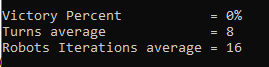
\includegraphics{img/pic_1.png}\\
\textbf{Resultados para el robot random}\\[0.5cm]

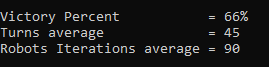
\includegraphics{img/pic_2.png}\\
\textbf{Resultados para el robot ni\~nera}\\[0.5cm]

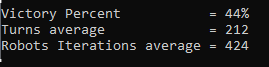
\includegraphics{img/pic_3.png}\\
\textbf{Resultados para el robot limpiador}\\[0.5cm]

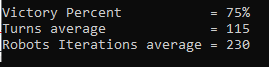
\includegraphics{img/pic_4.png}\\
\textbf{Resultados para el robot balanceado o equilibrado}\\[0.5cm]

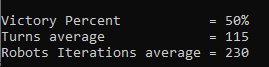
\includegraphics{img/pic_5.png}\\
\textbf{Resultados para el robot de trabajo en equipo}\\[0.5cm]
\end{center}


Los resultados para el robot random son los que esper\'abamos. En ninguna simulaci\'on logr\'o mantener el ambiente limpio y capturar los ni\~nos. En un promedio de solo 8 turnos ya ten\'ia el ambiente demasiado sucio. Dado que este tipo de robot \'unicamente se mueve a casillas v\'alidas que escoge al azar y limpia "de casualidad", estos resultados son m\'as que consistentes.

El robot ni\~nera obtuvo uno de los m\'as altos por cientos de victorias. En la mayor\'ia de los casos, la variaci\'on del ambiente le permiti\'o capturar a todos los ni\~nos antes de que se ensuciara m\'as de lo debido.

El robot limpiador fue el que obtuvo m\'as bajo promedio, pero fue el que m\'as turnos demor\'o en detener la simulaci\'on. El tener que dedicarse a limpiar como prioridad y no capturar los ni\~nos hace que estos sigan ensuciando hasta caer por debajo del l\'imite de limpieza. Sin embargo, en algunos casos, esta estrategia fue exitosa, ya que en estos los ni\~nos no ensuciaban demasiado en el momento de cambio de ambiente, y el robot pudo capturarlos.

El robot balanceado fue el que m\'as alto porcentaje tuvo. Viene dado por su estrategia de hacer lo mejor en el momento que se va a mover. Logr\'o una eficacia del 75\%. Sin embargo, hubo casos de fracaso. Lo cual puede venir dado por la cantidad de suciedad nueva que se genera en los cambios aleatorios y el movimiento de los ni\~nos.

Finalmente, el robot de trabajo en equipo, con una eficacia promedio del 50\%, logr\'o su objetivo en la mitad de los casos. Su promedio no tan alto puede venir dado a que eran solo dos robots en el ambiente. En ambientes donde se permitan m\'as robots, el n\'umero de cada "equipo" aumenta, haciendo m\'as eficaz su estrategia.\\

Podemos concluir que, menos del robot random, cada estrategia es v\'alida dependiendo de los cambios del ambiente. Como estos ocurren aleatoriamente, no podemos predecir cu\'ando y d\'onde un ni\~no va a ensuciar, a d\'onde se va a mover etc, por lo que la estrategia funciona si, casualmente, el ambiente es el "id\'oneo" para esta. El robot balanceado demostr\'o ser el m\'as eficaz. Pero tambi\'en existen casos donde su estrategia falla. Por otro lado, el robot de trabajo en equipo, podr\'ia ser tan eficiente como el balanceado si existen m\'as robots en el ambiente.\\\\

\section{Github}
En este \href{https://github.com/Alexx-4/Agentes-Haskell}{\textcolor{red}{\underline{enlace}}} podemos encontrar el repositorio del proyecto en Github.


\end{document}